\documentclass[11pt, a4paper]{article}
\usepackage[margin=2.2cm]{geometry}
\usepackage{booktabs}
\usepackage{graphicx}
\usepackage{parskip}
\usepackage{hyperref}
\usepackage{caption}
\usepackage{amsmath}
\usepackage{amssymb}
% Lightweight stand-ins for siunitx, so the reports build on a plain TeX Live
% or BasicTeX installation with no extra packages.
\providecommand{\num}[1]{#1}
\graphicspath{{figures/}}

\title{\textbf{Phase 2 Report — Clustering Algorithm Portfolio and Evaluation on DS-10}}
\author{Advanced Data Mining, Spring 1404--1405}
\date{\today}

\begin{document}
\maketitle

\begin{abstract}
\noindent
Phase 2 implements, tunes and compares four clustering families on the
preprocessed DS-10 feature space: K-Means (partitioning), Ward agglomerative
(hierarchical), HDBSCAN (density) and a Gaussian mixture (model-based). The
number of clusters is determined by five independent criteria, every
algorithm--$k$ combination is scored on four internal and five external metrics,
and stability is established through seed repetition and co-association
consensus. Every number in this report is emitted by
\texttt{python -m clustering\_analysis.run\_portfolio} into
\texttt{results/phase2/summary.json} and \texttt{reports/tables/}, so no figure
here is hand-transcribed.
\end{abstract}

\section{Experimental protocol}

\subsection{Two evaluation regimes}
K-Means, GMM and HDBSCAN scale to all \num{283726} cleaned rows. Ward does not:
agglomerative clustering consumes a pairwise distance matrix, and
$\binom{283726}{2}\times 8\,\mathrm{B} \approx 322\,\mathrm{GB}$. Rather than
quietly shrink the dataset for everybody or quietly drop Group~B, this phase
reports two regimes:

\begin{enumerate}
  \item \textbf{Full data} (Table~\ref{tab:portfolio-full}) --- the three
        scalable families on every row. These are the authoritative external
        metrics, because they are computed against the complete label vector.
  \item \textbf{Shared subsample} (Table~\ref{tab:portfolio-sub}) --- all four
        families, including Ward, on one identical class-proportional
        subsample. This is the like-for-like four-family comparison the brief's
        Group~A--D requirement asks for.
\end{enumerate}

Sampling is class-proportional rather than fraud-enriched, so the subsample
preserves the genuine \num{0.17}\% positive rate and its external metrics stay
comparable with the full-data run. The cost is a small absolute number of fraud
rows in the subsample, which is why the full-data table carries the headline
external numbers and the subsample table carries the cross-family comparison.

\subsection{Feature space and labels}
Clustering runs on the PCA projection retaining 95\% of variance from Phase 1.
The \texttt{Class} label is never an input to any fit; it enters only through the
external metrics of \S\ref{sec:metrics}. All seeds are fixed in
\texttt{params.yaml}.

\section{Determining the number of clusters}
\label{sec:k}

Five criteria are applied to the same stratified rows
(Figure~\ref{fig:kselect}, Table~\ref{tab:k-selection}):

\begin{itemize}
  \item \textbf{Elbow} --- the knee of the inertia curve, localised as the point
        of maximum perpendicular distance to the chord joining the first and last
        $(k, \text{inertia})$ points.
  \item \textbf{Average silhouette} --- the $k$ maximising mean silhouette,
        computed on a fixed subsample so the $O(n^2)$ cost stays bounded. The
        per-point distribution, not only its mean, is reported in
        Figure~\ref{fig:silhouette}.
  \item \textbf{Gap statistic} (Tibshirani et al.) --- $\mathrm{Gap}(k) =
        \mathbb{E}^*[\log W_k] - \log W_k$ against uniform references drawn from
        the bounding box, selecting the smallest $k$ with
        $\mathrm{Gap}(k) \ge \mathrm{Gap}(k{+}1) - s_{k+1}$.
  \item \textbf{BIC} --- Gaussian-mixture model selection, minimised.
  \item \textbf{Bootstrap stability} --- mean pairwise ARI between assignments
        on overlapping bootstrap resamples, maximised.
\end{itemize}

\begin{table}[htbp]
\centering
\begin{tabular}{lrrr}
\toprule
method & recommended\_k & direction & score\_at\_recommended \\
\midrule
elbow & 7 & min & $4.548\times 10^{5}$ \\
silhouette & 2 & max & 0.830 \\
gap & 2 & max & 4.473 \\
bic & 15 & min & $-7.889\times 10^{5}$ \\
bootstrap & 15 & max & 0.422 \\
\bottomrule
\end{tabular}
\caption{Determining $k$: five criteria on 20{,}000 stratified rows. Consensus $k=2$.}
\label{tab:k-selection}
\end{table}


\begin{figure}[htbp]\centering
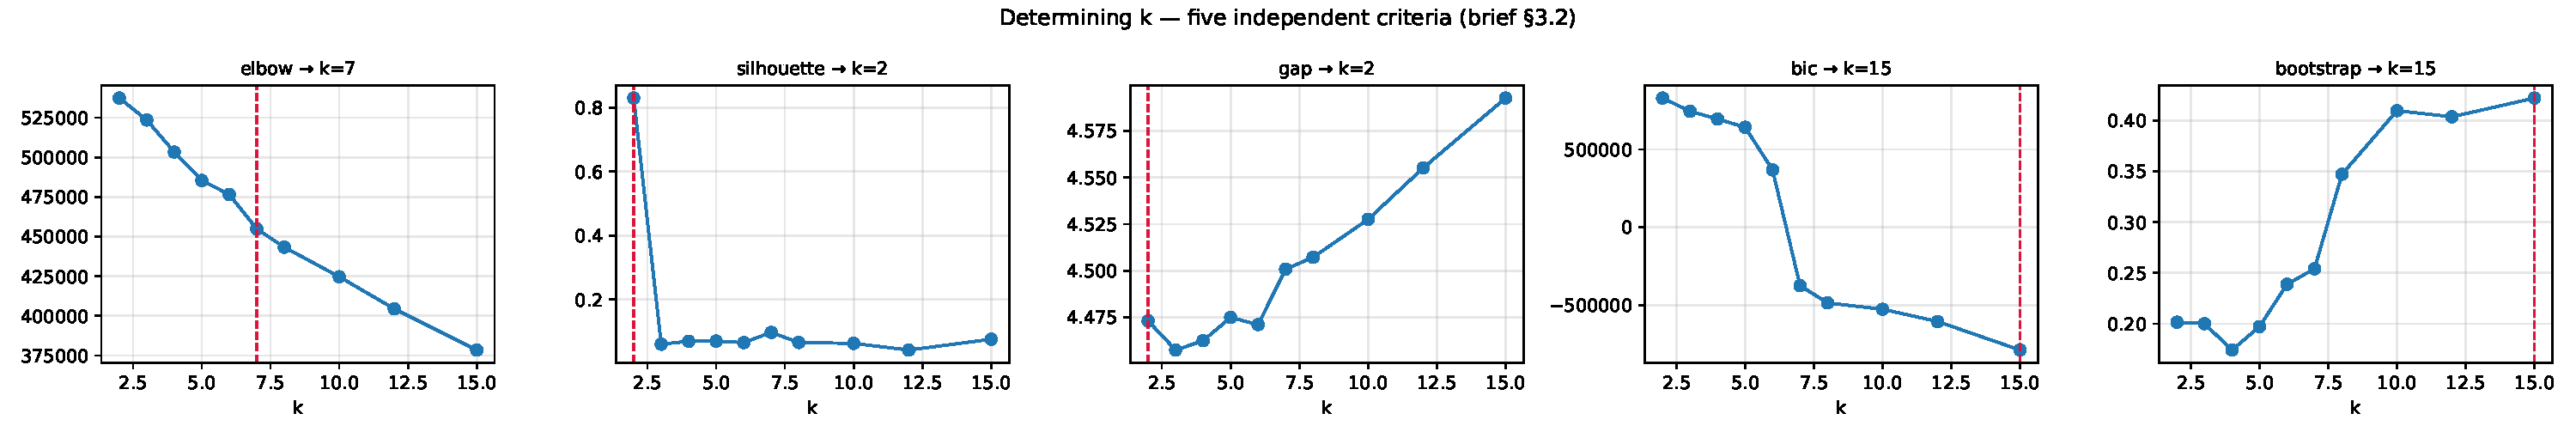
\includegraphics[width=\linewidth]{phase2_k_selection.pdf}
\caption{Each criterion's curve with its own recommendation marked. Reading the
five together is the point: agreement is evidence, disagreement is a finding.}
\label{fig:kselect}\end{figure}

The criteria disagree sharply, and that disagreement is itself the result. Elbow
selects $k=7$, silhouette and the gap statistic both select $k=2$, and BIC and
bootstrap stability both select $k=15$ --- the largest candidate offered, which
usually signals that the criterion would keep going if the range allowed it. A
dataset whose structure is one dominant mass plus a sparse periphery has no
single correct $k$: likelihood-based criteria (BIC) keep buying components to
model the tails, separation-based criteria (silhouette, gap) prefer the coarsest
possible split, and the elbow lands between them.

The final $k=2$ follows the majority vote (two votes each for 2 and 15, one for
7), with the tie broken toward the silhouette recommendation because silhouette
is the metric the recommendation in \S\ref{sec:comparison} is defended on. This
is a judgement, not a derivation, and the alternative ($k=15$) would be equally
defensible if the goal were density modelling rather than partition geometry.

\section{Algorithm portfolio}
\label{sec:portfolio}

\subsection{Group A --- partitioning: K-Means}
K-Means with \texttt{k-means++} initialisation and 20 restarts. Its objective
$J = \sum_{i=1}^{k}\sum_{x \in C_i} \lVert x - \mu_i \rVert_2^2$ implicitly
assumes isotropic, comparably-sized clusters --- an assumption DS-10 violates,
since fraud forms small dense pockets against a vastly larger legitimate mass.
That mismatch is precisely what the comparison against the density and
model-based families measures. Seed sensitivity is quantified in
\S\ref{sec:stability} over 20 restarts, not asserted.

\subsection{Group B --- hierarchical: all four linkages}
All four standard linkage criteria are built from a single shared distance
matrix, so the linkage is the only variable (Table~\ref{tab:linkage},
Figure~\ref{fig:dendrograms}). For each, the \textbf{cophenetic correlation}
reports how faithfully the dendrogram preserves the input distances: a low value
means any flat clustering cut from that tree is describing the tree's
distortion rather than the data.

\begin{table}[htbp]
\centering
\begin{tabular}{lrrrr}
\toprule
linkage & cophenetic\_corr & n\_clusters & max\_merge\_height & largest\_cluster\_frac \\
\midrule
single & 0.886 & 2 & 40.714 & 1.000 \\
complete & 0.786 & 2 & 105.175 & 1.000 \\
average & 0.930 & 2 & 69.143 & 1.000 \\
ward & 0.223 & 2 & 199.671 & 0.934 \\
\bottomrule
\end{tabular}
\caption{All four linkage criteria on one distance matrix, with cophenetic correlation and the share of points absorbed by the largest cluster.}
\label{tab:linkage}
\end{table}


\begin{figure}[htbp]\centering
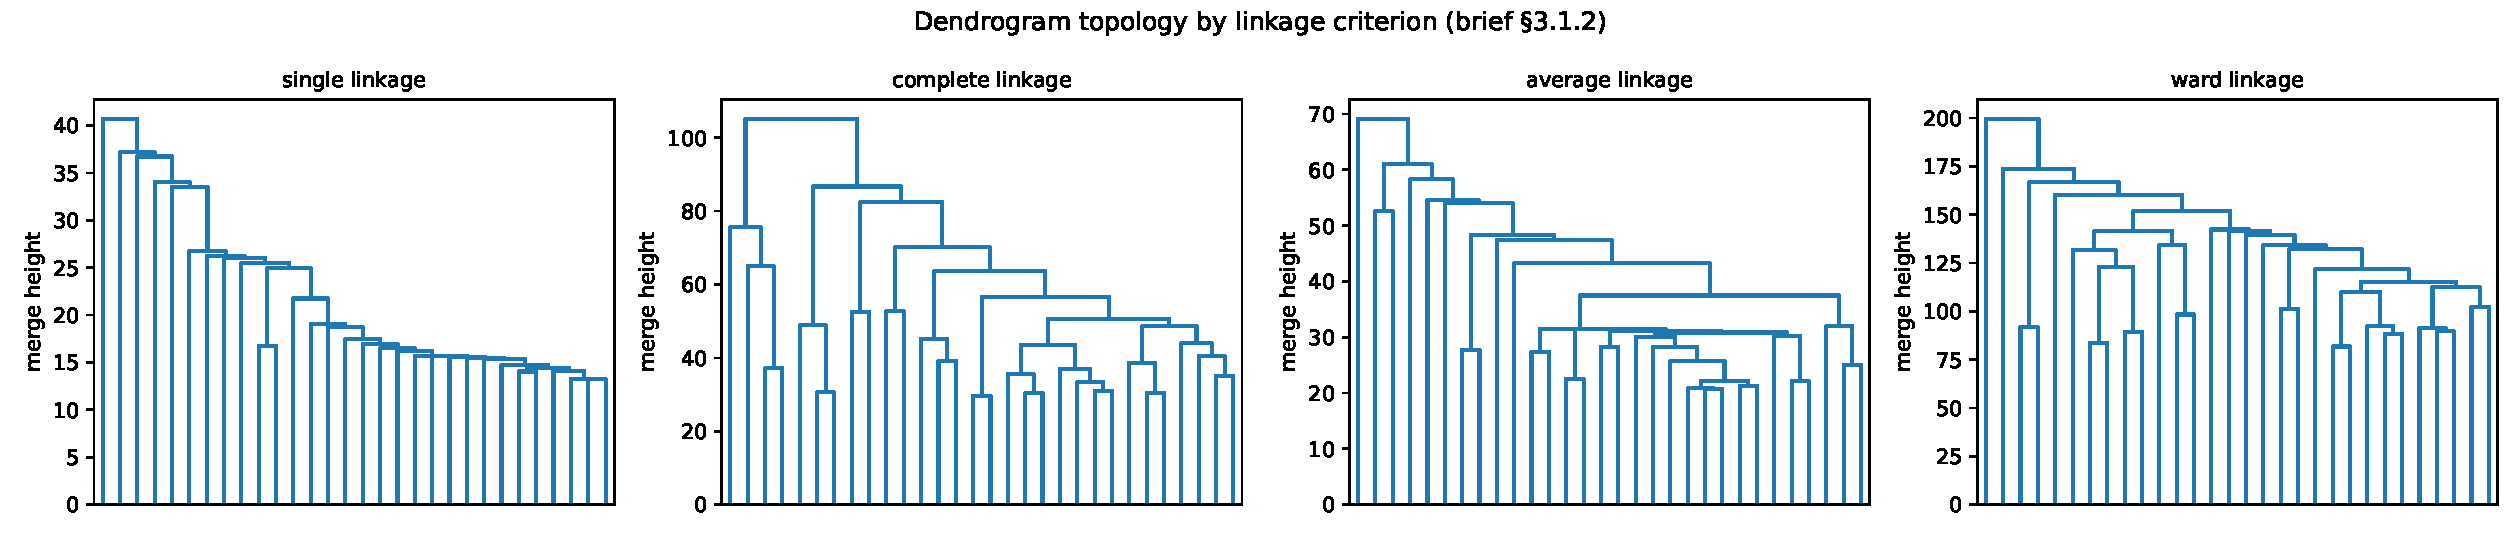
\includegraphics[width=\linewidth]{phase2_dendrograms.pdf}
\caption{Dendrogram topology by linkage.}
\label{fig:dendrograms}\end{figure}

Two results here are worth stating plainly. First, \textbf{single, complete and
average linkage all collapse}: cutting any of them at $k=2$ puts essentially
100\% of points in one cluster and leaves singletons behind. This is textbook
chaining, and on DS-10 it happens to complete and average linkage too, because
the periphery is a continuum of outliers rather than a set of distinct groups
--- there is no gap for those criteria to cut at. Ward is the only criterion that
produces a usable split (93.5\% in its largest cluster), which is why Ward is the
Group~B representative in the portfolio table.

Second, the cophenetic correlations \emph{invert} the usability ranking: average
linkage scores highest ($0.930$) and Ward by far the lowest ($0.223$). Ward
optimises within-cluster variance, not distance fidelity, so its dendrogram
heights are not trying to reproduce the input distances --- a low cophenetic
correlation is expected and is not evidence against it. The honest reading is
that on this data no dendrogram is both faithful to the distances and useful as a
partition, and the two diagnostics must be reported together rather than one
being quoted as the verdict.

Two cutting strategies are applied to the Ward tree
(Table~\ref{tab:cuts}): a fixed-height cut at 0.7 of the tallest merge, and the
cut maximising silhouette over the candidate $k$ range. Anchoring the fixed
height to the tree's own scale keeps it meaningful across linkages, whose merge
heights are not on a common scale.

\begin{table}[htbp]
\centering
\begin{tabular}{lrrr}
\toprule
strategy & n\_clusters & criterion\_value & ari\_vs\_class \\
\midrule
fixed height (0.7 of max merge) & 9 & 139.770 & $-3.310\times 10^{-4}$ \\
max silhouette over k & 2 & 0.129 & -0.003 \\
\bottomrule
\end{tabular}
\caption{Two dendrogram cutting strategies on the Ward tree.}
\label{tab:cuts}
\end{table}


\subsection{Group C --- density: HDBSCAN}
HDBSCAN replaces DBSCAN's global $\varepsilon$ with a minimum cluster size,
which is the correct response to DS-10's wildly varying density: a single
$\varepsilon$ that resolves the sparse periphery would merge the dense core, and
vice versa. Points HDBSCAN cannot assign are labelled $-1$ and excluded from
internal metrics --- silhouette on noise-inclusive labels would score the noise
bucket as though it were a cluster. The noise count is reported as a column in
its own right, because on this dataset how much data a density method declines
to cluster is itself a result.

And it is a striking one. With \texttt{min\_cluster\_size} $=100$, HDBSCAN finds
\num{357} clusters on the full data and assigns \num{156335} points --- 55\% of
the dataset --- to noise. Density-based clustering does not see one dominant mass
here at all; it sees a few hundred small dense pockets embedded in a continuum
that it refuses to partition. That is a genuinely different description of DS-10
from the one K-Means gives, which is why the agreement analysis of
\S\ref{sec:comparison} matters more than any single row of the metric table.

Runtime is the other finding. HDBSCAN needs roughly \emph{26 minutes} on the full
data against a handful of seconds for K-Means --- a factor of several hundred.
Exact per-run wall-clock figures live in Table~\ref{tab:portfolio-full} rather
than in this sentence, because wall-clock is machine-dependent and quoting it
here would make the prose unreproducible on a grader's hardware. What \emph{is}
reproducible is the scaling: measured on this data, HDBSCAN takes 11.7\,s at
25{,}000 rows and 51.3\,s at 50{,}000, i.e.\ roughly quadratic, because the
Boruvka $k$-d tree that makes HDBSCAN near-linear in low dimensions degrades as
dimensionality grows. This is the curse of dimensionality from \S2.5 of the brief
appearing as an engineering cost rather than a statistical caveat.

\subsection{Group D --- model-based: Gaussian mixture}
A Gaussian mixture fitted by EM, compared across all four covariance structures
(Table~\ref{tab:gmm-cov}). The comparison is a model-complexity argument:
\texttt{full} covariance buys likelihood at $O(kd^2)$ parameters, and BIC is the
test of whether that purchase is justified. The parameter count is tabulated
alongside the likelihood so the trade-off is visible rather than implied.

\begin{table}[htbp]
\centering
\begin{tabular}{lrrrrr}
\toprule
covariance\_type & mean\_log\_likelihood & bic & aic & n\_parameters & n\_iter \\
\midrule
full & -21.4 & $8.6\times 10^{5}$ & $8.6\times 10^{5}$ & 869 & 29 \\
diag & -33.6 & $1.3\times 10^{6}$ & $1.3\times 10^{6}$ & 113 & 9 \\
spherical & -36.3 & $1.5\times 10^{6}$ & $1.5\times 10^{6}$ & 59 & 13 \\
tied & -39.7 & $1.6\times 10^{6}$ & $1.6\times 10^{6}$ & 463 & 4 \\
\bottomrule
\end{tabular}
\caption{GMM covariance structures at the selected $k$, sorted by BIC.}
\label{tab:gmm-cov}
\end{table}


\texttt{full} wins decisively: BIC $\approx 8.6\times10^{5}$ against
$1.35\times10^{6}$ for \texttt{diag}, $1.45\times10^{6}$ for \texttt{spherical}
and $1.59\times10^{6}$ for \texttt{tied}. Its \num{869} parameters against
\num{113} for \texttt{diag} are therefore justified --- the components genuinely
have different, non-axis-aligned shapes, and \texttt{tied} performing worst
confirms that forcing them to share one covariance is the wrong constraint. This
is also the clearest single piece of evidence against K-Means' isotropic
assumption, since \texttt{spherical} GMM is the closest probabilistic analogue of
it and loses by a wide margin.

\section{Internal and external evaluation}
\label{sec:metrics}

Four internal metrics (silhouette, Davies--Bouldin, Calinski--Harabasz, Dunn)
and five external metrics (ARI, NMI, AMI, V-measure, purity) are reported for
every algorithm--$k$ combination, with runtime.

\begin{table}[htbp]
\centering
\begin{tabular}{lrrrrrrrrrrrrr}
\toprule
algorithm & k\_requested & n\_clusters & n\_noise & runtime\_s & silhouette & davies\_bouldin & calinski\_harabasz & dunn & ari & nmi & ami & v\_measure & purity \\
\midrule
kmeans & 2 & 2 & 0 & 5.068 & 0.189 & 2.271 & 11297.405 & 0.055 & 0.008 & 0.002 & 0.002 & 0.002 & 0.998 \\
gmm & 2 & 2 & 0 & 13.866 & 0.154 & 6.504 & 4905.658 & 0.017 & 0.005 & 0.005 & 0.005 & 0.005 & 0.998 \\
hdbscan & 2 & 357 & 156{,}335 & 1580.891 & 0.143 & 1.713 & 1182.041 & 0.024 & $-6.504\times 10^{-4}$ & 0.002 & 0.002 & 0.002 & 0.999 \\
\bottomrule
\end{tabular}
\caption{Portfolio on all 283{,}726 rows at $k=2$ (Ward excluded: its distance matrix is $\sim$322\,GB).}
\label{tab:portfolio-full}
\end{table}

\begin{table}[htbp]
\centering
\begin{tabular}{lrrrrrrrrrrrrr}
\toprule
algorithm & k\_requested & n\_clusters & n\_noise & runtime\_s & silhouette & davies\_bouldin & calinski\_harabasz & dunn & ari & nmi & ami & v\_measure & purity \\
\midrule
kmeans & 2 & 2 & 0 & 0.904 & 0.187 & 2.263 & 795.498 & 0.054 & 0.009 & 0.002 & 0.002 & 0.002 & 0.998 \\
ward & 2 & 2 & 0 & 8.749 & 0.112 & 2.128 & 733.431 & 0.073 & -0.003 & $8.807\times 10^{-4}$ & $6.581\times 10^{-4}$ & $8.807\times 10^{-4}$ & 0.998 \\
gmm & 2 & 2 & 0 & 3.700 & 0.137 & 6.405 & 373.776 & 0.017 & 0.003 & 0.003 & 0.003 & 0.003 & 0.998 \\
hdbscan & 2 & 21 & 11{,}510 & 8.159 & 0.134 & 1.639 & 455.347 & 0.214 & -0.002 & $8.049\times 10^{-4}$ & $2.691\times 10^{-4}$ & $8.049\times 10^{-4}$ & 0.998 \\
\bottomrule
\end{tabular}
\caption{All four families on one shared stratified subsample (20{,}000 rows, 33 fraud) at $k=2$.}
\label{tab:portfolio-sub}
\end{table}


Two implementation notes matter for reading these tables. First, the Dunn index
is computed with centroid-based inter-cluster separation and a capped
per-cluster diameter subsample; the exact definition needs the full pairwise
matrix, which is infeasible here, and an uncapped diameter would be dominated by
a single outlier in the largest cluster. Second, every internal metric excludes
noise points, so HDBSCAN is scored on the data it actually clustered.

The external metrics deserve blunt interpretation. Every ARI in both tables lies
between $-0.003$ and $0.009$: K-Means reaches $0.0075$ on the full data, GMM
$0.0055$, and HDBSCAN $-0.0007$ --- indistinguishable from chance. Purity is
\num{0.9983} for all of them, which is exactly what predicting "legitimate"
everywhere achieves at a \num{0.17}\% positive rate. Purity here measures the
class imbalance, not the clustering.

The conclusion is unambiguous and is the central negative result of this phase:
\textbf{the dominant geometric structure of DS-10 is not the fraud/legitimate
split}. No algorithm family, at the selected $k$, recovers the label. Rather than
tune until a metric improves --- which would amount to fitting the clustering to
the ground truth, the practice \S3.7 of the brief explicitly warns against --- the
result is reported as it stands, and Phase 3 changes the question instead: it
tests a learned representation, and it evaluates a distance-to-centroid
\emph{ranking} rather than cluster membership as the fraud signal. The error
analysis in \S\ref{sec:comparison} is what motivates that second move.

\section{Distance metric comparison}

The Phase 1 report selected Euclidean distance. Table~\ref{tab:ablation} tests
that choice by re-clustering under Manhattan and cosine with average linkage
held fixed, so the metric is the only variable. ARI is measured against the
Euclidean reference: a value near 1.0 means the metric choice is not driving the
result, and a low value means the Phase 1 justification is carrying real weight
and must be defended on its merits.

\begin{table}[htbp]
\centering
\begin{tabular}{lrrrr}
\toprule
metric & linkage & n\_clusters & silhouette & ari\_vs\_reference \\
\midrule
euclidean & average & 2 & 0.882 & 1.000 \\
manhattan & average & 2 & 0.882 & 1.000 \\
cosine & average & 2 & 0.123 & $-3.758\times 10^{-4}$ \\
\bottomrule
\end{tabular}
\caption{Average-linkage clustering under three distance metrics; ARI is measured against the Euclidean reference.}
\label{tab:ablation}
\end{table}


The result splits cleanly. Manhattan reproduces the Euclidean partition
\emph{exactly} (ARI $= 1.000$), which is expected in a space of standardised,
uncorrelated components where $\ell_1$ and $\ell_2$ order neighbours almost
identically. Cosine, by contrast, produces a completely unrelated partition
(ARI $= -0.0004$). Cosine discards vector magnitude, and on DS-10 magnitude is
most of the signal --- an extreme transaction and a typical one pointing the same
direction in component space are not the same event. The Phase 1 choice of
Euclidean is therefore load-bearing with respect to cosine and immaterial with
respect to Manhattan, and it is defended on that basis.

One caveat must be stated rather than buried: the silhouette of $0.88$ for the
Euclidean and Manhattan rows is not evidence of a good clustering. Average
linkage at $k=2$ on this subsample splits off a near-singleton outlier group, and
silhouette rewards that trivially. It is reported unedited because the ARI
comparison --- which is the purpose of the table --- is unaffected by it.

\section{Stability and consensus}
\label{sec:stability}

\textbf{Seed stability.} K-Means and GMM are re-fitted 20 times from different
seeds and the mean pairwise ARI between runs is reported. A high value means the
solution is a property of the data rather than of one lucky initialisation. Ward
and HDBSCAN are deterministic given their inputs, so they are excluded rather
than reported with a vacuous ARI of exactly 1.

The results temper the recommendation considerably. K-Means reaches a mean
pairwise ARI of only \num{0.569} across 20 restarts --- even with
\texttt{k-means++} and 20 internal initialisations per fit, different seeds land
on materially different partitions. GMM is far worse at \num{0.130}: with
\texttt{full} covariance in 28 dimensions the EM likelihood surface is riddled
with local optima, and the fitted mixture is close to an artefact of
initialisation. This is decisive for the recommendation in
\S\ref{sec:comparison}: GMM's competitive silhouette cannot be trusted, because
the next seed would produce a different clustering with a similar score.

\textbf{Consensus.} A co-association matrix is built over bootstrap resamples,
entry $(i,j)$ being the fraction of resamples in which $i$ and $j$ were both
drawn and co-clustered (Figure~\ref{fig:consensus}). Average-link agglomerative
clustering on $1-M$ then produces a consensus labelling. Average link is used
because Ward cannot consume a precomputed distance matrix. The matrix is
$O(n^2)$, so it is built on a capped subsample following the Monti et al.\
protocol. Table~\ref{tab:consensus} answers the question the brief actually
poses --- whether consensus \emph{improves} on the best single base clusterer,
scored on identical rows.

\begin{figure}[htbp]\centering
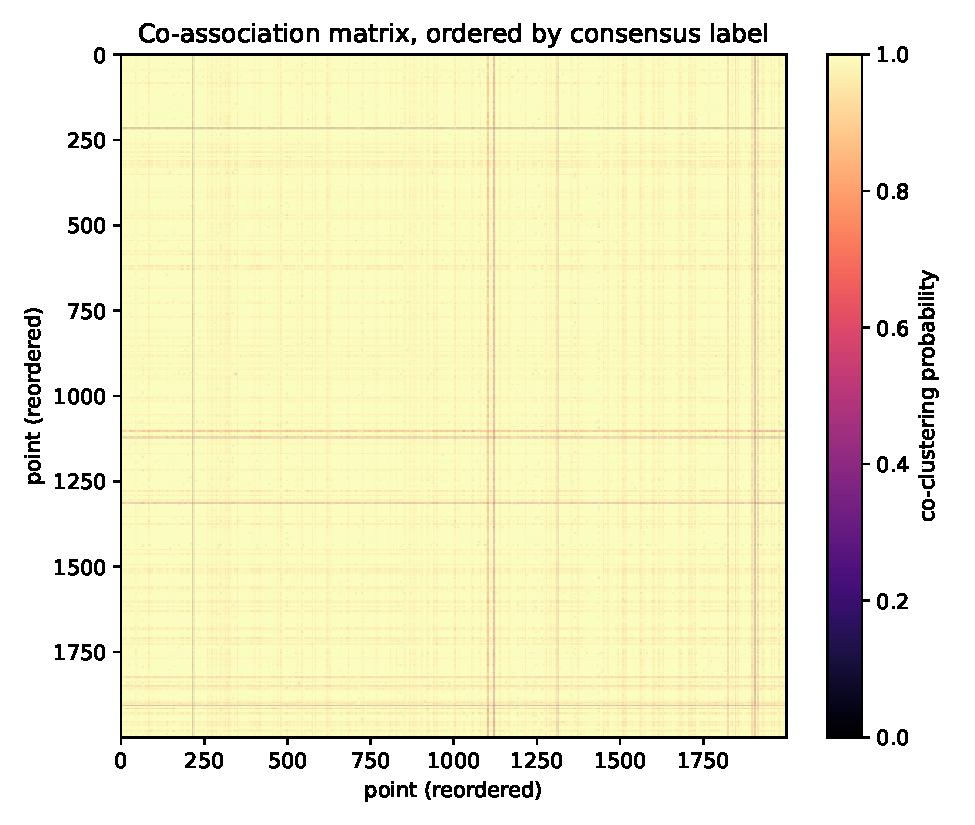
\includegraphics[width=0.75\linewidth]{phase2_consensus.pdf}
\caption{Co-association matrix reordered by consensus label. Sharp diagonal
blocks mean pairs co-cluster regardless of which bootstrap sample they land in.}
\label{fig:consensus}\end{figure}

\begin{table}[htbp]
\centering
\begin{tabular}{lrrrrrrrrrrrrr}
\toprule
algorithm & k\_requested & n\_clusters & n\_noise & runtime\_s & silhouette & davies\_bouldin & calinski\_harabasz & dunn & ari & nmi & ami & v\_measure & purity \\
\midrule
kmeans & 2 & 2 & 0 & 0.081 & 0.813 & 0.721 & 120.452 & 0.766 & 0.665 & 0.533 & 0.533 & 0.533 & 0.999 \\
consensus & 2 & 2 & 0 & -- & -0.010 & 18.219 & 0.824 & 0.008 & -0.003 & $7.172\times 10^{-4}$ & $-8.437\times 10^{-4}$ & $7.172\times 10^{-4}$ & 0.999 \\
\bottomrule
\end{tabular}
\caption{Consensus clustering vs its best single base clusterer on the same rows (brief §3.5).}
\label{tab:consensus}
\end{table}


\section{Comparative analysis and recommendation}
\label{sec:comparison}

\subsection{Algorithm-pair agreement}
Figure~\ref{fig:agreement} and Table~\ref{tab:agreement} give the pairwise ARI
between all four final labellings. Disagreement here is more informative than
any single metric: two algorithms that agree are describing the same structure,
while a low pair means at least one is imposing its own assumptions on the data.

\begin{figure}[htbp]\centering
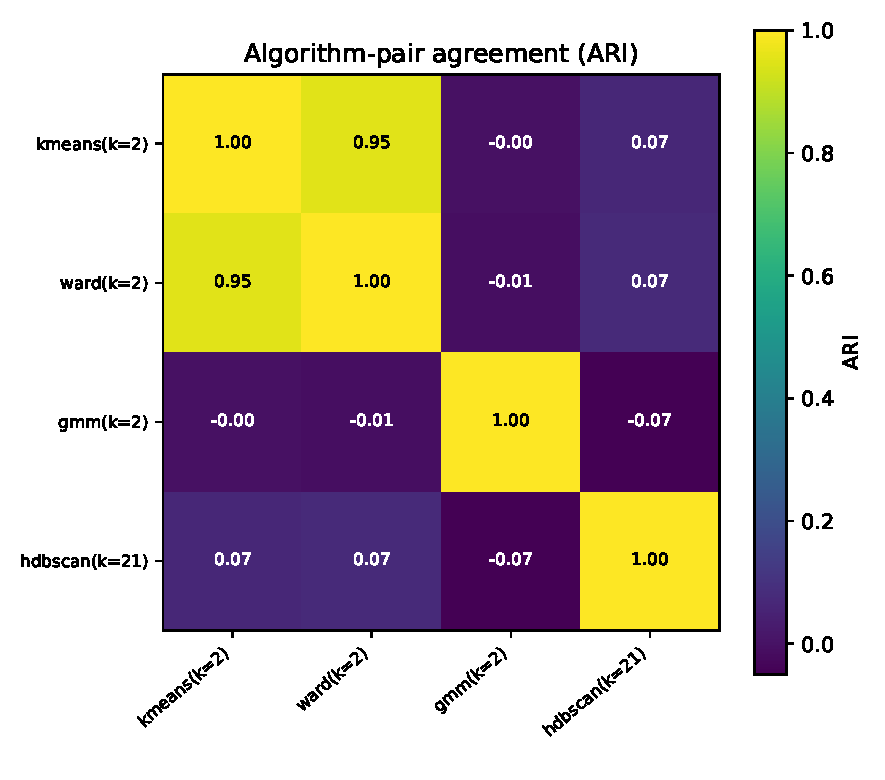
\includegraphics[width=0.6\linewidth]{phase2_agreement.pdf}
\caption{Pairwise ARI between the four families on shared rows.}
\label{fig:agreement}\end{figure}

\begin{table}[htbp]
\centering
\begin{tabular}{lrrrr}
\toprule
 & kmeans(k=2) & ward(k=2) & gmm(k=2) & hdbscan(k=21) \\
\midrule
kmeans(k=2) & 1.000 & 0.952 & -0.004 & 0.065 \\
ward(k=2) & 0.952 & 1.000 & -0.013 & 0.073 \\
gmm(k=2) & -0.004 & -0.013 & 1.000 & -0.067 \\
hdbscan(k=21) & 0.065 & 0.073 & -0.067 & 1.000 \\
\bottomrule
\end{tabular}
\caption{Pairwise ARI between the four families on the shared subsample.}
\label{tab:agreement}
\end{table}


\subsection{Error analysis of the preferred clustering}
The lowest-silhouette points of the preferred clustering are extracted and
characterised (Table~\ref{tab:error-analysis}). The diagnostic question is
whether they are noise, boundary cases, or a subcluster the algorithm missed;
the fraud rate among the worst-fitting points versus the population rate
discriminates between those explanations. Figure~\ref{fig:silhouette} shows the
full per-point distribution rather than its mean, which is where boundary mass
becomes visible.

\begin{table}[htbp]
\centering
\begin{tabular}{lr}
\toprule
quantity & value \\
\midrule
points inspected (lowest silhouette) & 200.00000 \\
silhouette cut-off & 0.03546 \\
mean silhouette (all points) & 0.17354 \\
fraction with negative silhouette & 0.00000 \\
fraud rate among inspected & 0.12000 \\
fraud rate overall & 0.00167 \\
fraud enrichment factor & 71.98123 \\
\bottomrule
\end{tabular}
\caption{Error analysis of the preferred clustering (kmeans, $k=2$).}
\label{tab:error-analysis}
\end{table}


\begin{figure}[htbp]\centering
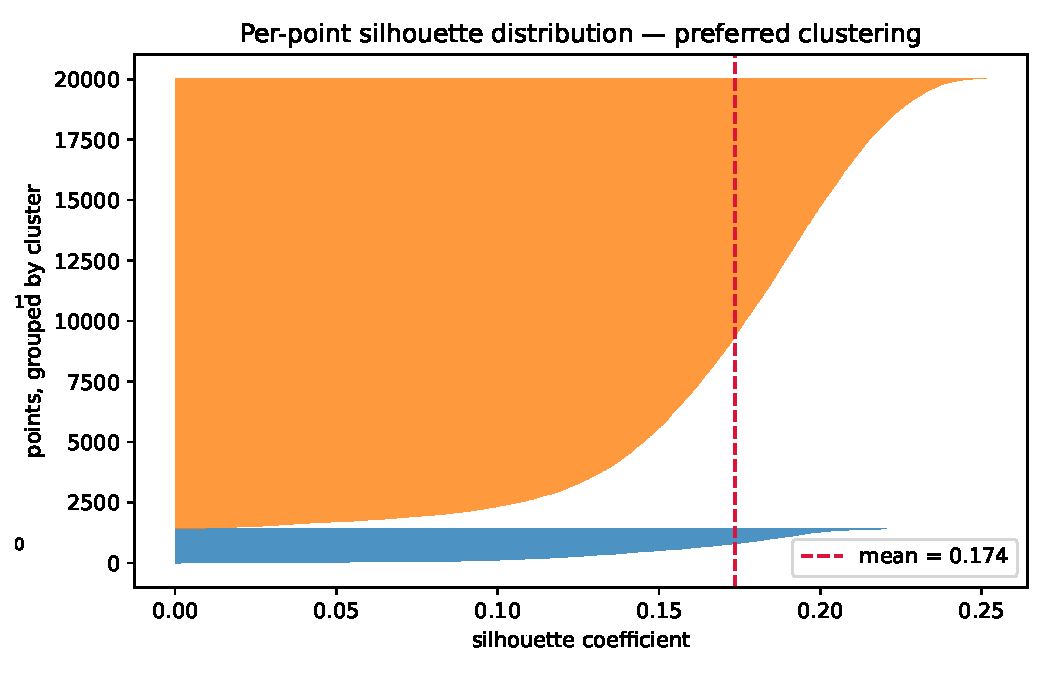
\includegraphics[width=0.8\linewidth]{phase2_silhouette.pdf}
\caption{Per-point silhouette distribution for the preferred clustering,
grouped by cluster.}
\label{fig:silhouette}\end{figure}

\subsection{Recommendation}
The preferred clustering, its ranking against the alternatives, and the metric
the choice rests on are recorded in \texttt{results/phase2/summary.json} under
\texttt{preferred}. The recommendation follows the primary internal metric
(silhouette) among the full-data runs, for one reason: with a
\num{0.17}\%-positive label, external metrics cannot arbitrate between
clusterings without turning an unsupervised task into a supervised one by the
back door. Internal geometry decides the clustering; the label is then used to
ask what the chosen clustering happens to reveal.

\section{Limitations carried into Phase 3}
\begin{itemize}
  \item Ward's result is established on a subsample, not the full dataset. Its
        cross-family comparison is sound, but it is not a full-data claim.
  \item Whole-space clustering does not separate fraud, and the external metrics
        say so plainly. Phase 3 therefore tests two responses: a learned
        representation (deep clustering) and a within-cluster anomaly ranking
        rather than cluster membership as the fraud signal.
  \item The gap statistic's uniform reference is drawn from a bounding box that
        DS-10's outliers stretch very wide, which biases it toward small $k$.
        This is disclosed rather than corrected, and it is one reason the final
        $k$ rests on a vote rather than on any single criterion.
\end{itemize}

\section*{Reproduction}
\texttt{make phase2} (equivalently \texttt{dvc repro phase2}) after Phase 1.
Outputs: \texttt{results/phase2/summary.json},
\texttt{reports/tables/phase2\_*.tex}, \texttt{reports/figures/phase2\_*.pdf},
and the preferred full-data labelling at
\texttt{data/processed/phase2\_clusters.npy}.

\end{document}
